\documentclass{standalone}
\usepackage{tikz}
\usetikzlibrary{patterns, positioning}
\usepackage[sfdefault]{ClearSans} %% option 'sfdefault' activates Clear Sans as the default text font
\usepackage[T1]{fontenc}

\begin{document}
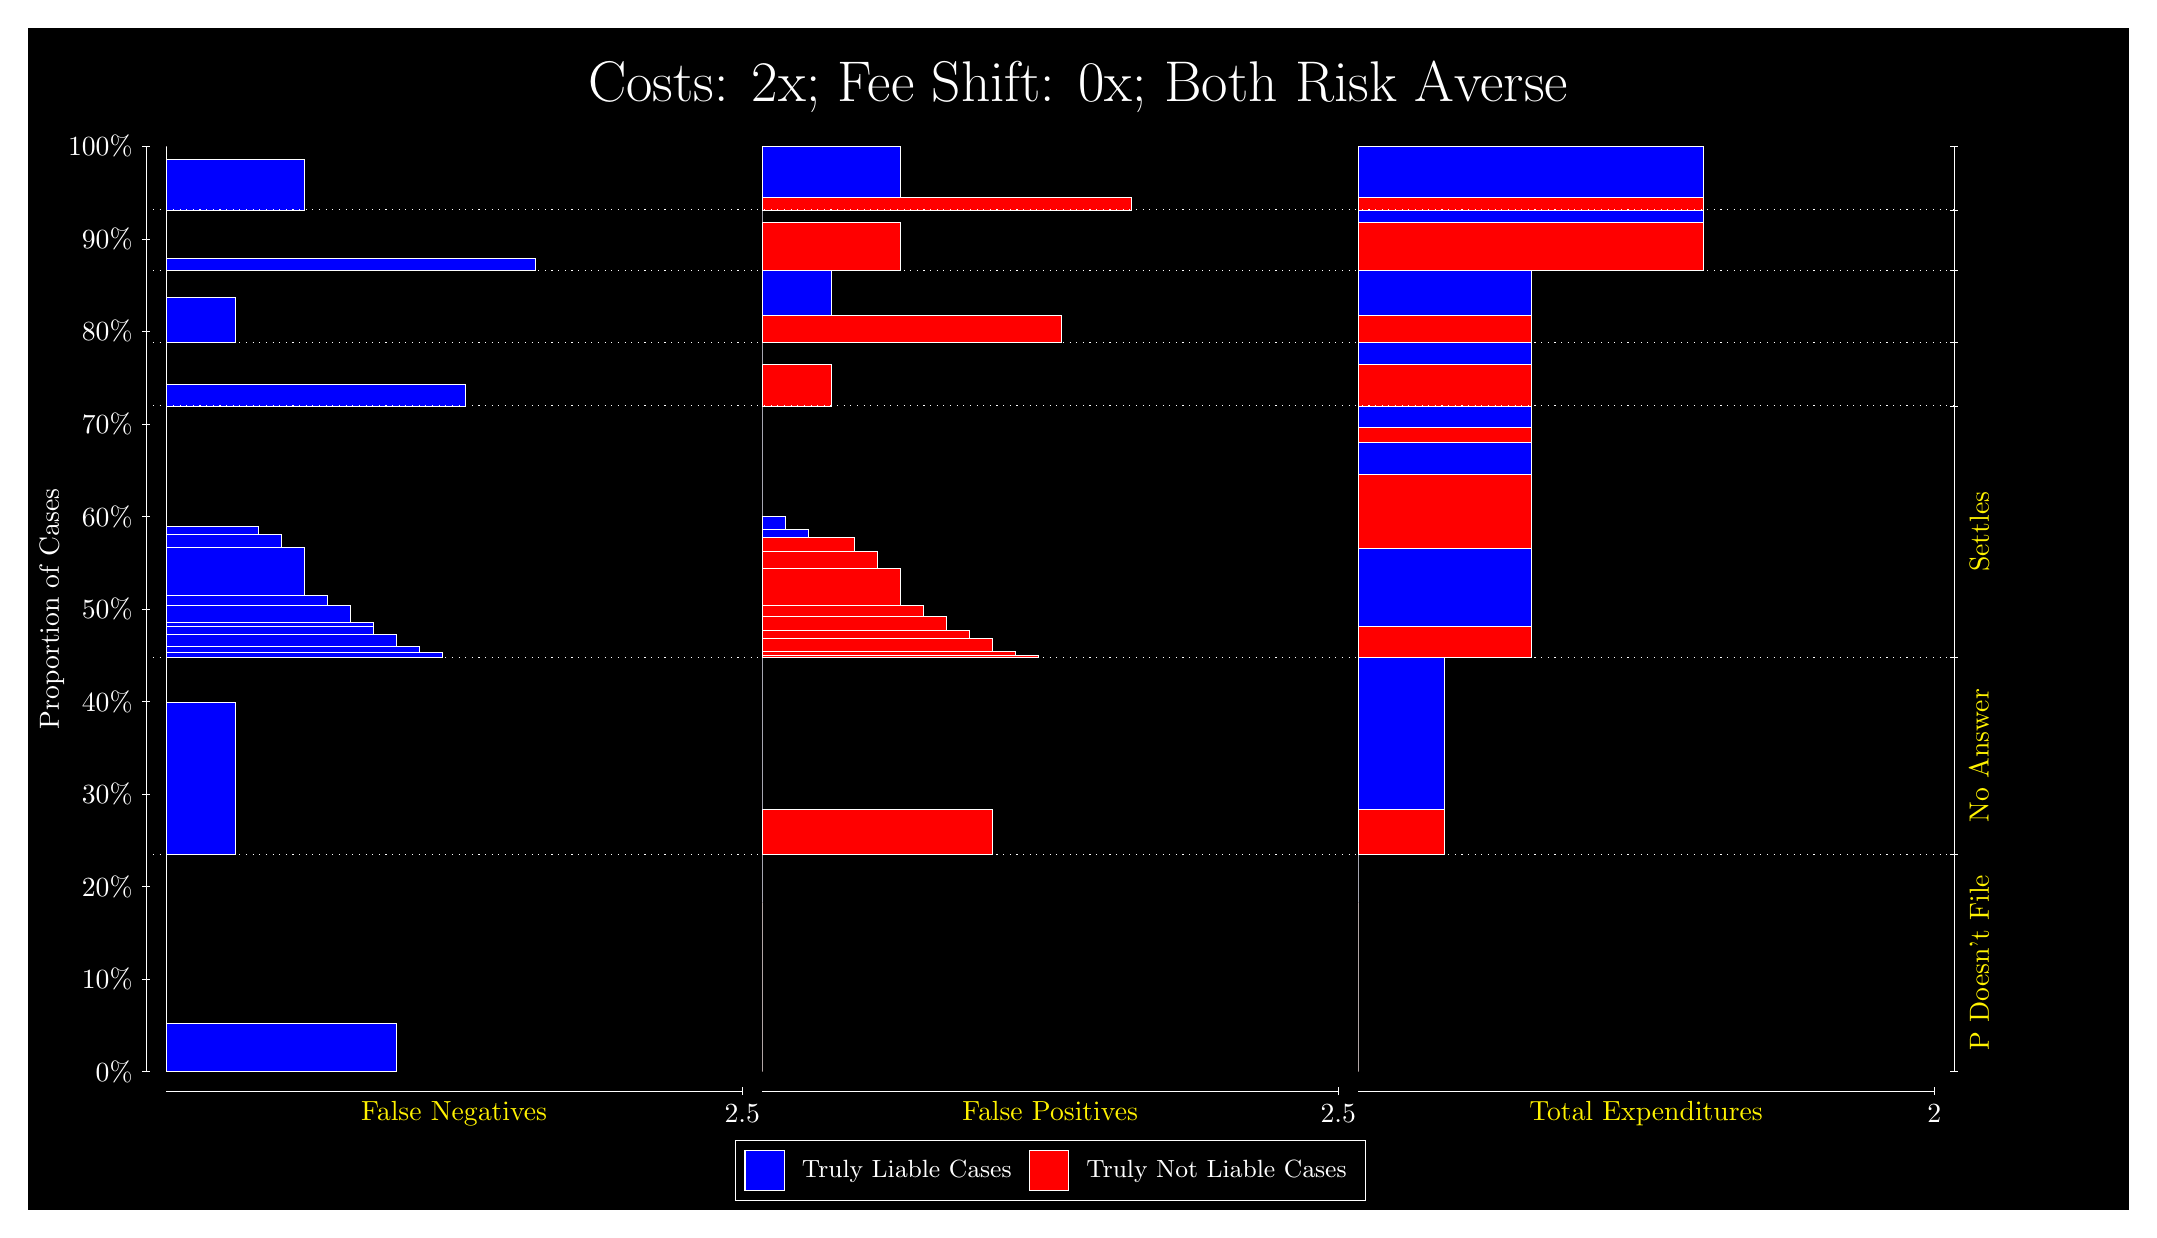
\begin{tikzpicture}
\draw[fill=black] (0,0) rectangle (26.667,15);
\draw[text=white] (0,13.5) rectangle (26.667,15) node[midway] {\huge Costs: 2x; Fee Shift: 0x; Both Risk Averse};
\draw[white, very thin] (1.5,1.75) -- (1.5,13.5);
\node[rotate=90, text=white, anchor=center] at (0.3, 7.625) {Proportion of Cases};
\draw[white, very thin] (1.45,1.75) -- (1.55,1.75);
\node[text=white, anchor=east] at (1.45, 1.75) {0\%};
\draw[white, very thin] (1.45,2.925) -- (1.55,2.925);
\node[text=white, anchor=east] at (1.45, 2.925) {10\%};
\draw[white, very thin] (1.45,4.1) -- (1.55,4.1);
\node[text=white, anchor=east] at (1.45, 4.1) {20\%};
\draw[white, very thin] (1.45,5.275) -- (1.55,5.275);
\node[text=white, anchor=east] at (1.45, 5.275) {30\%};
\draw[white, very thin] (1.45,6.45) -- (1.55,6.45);
\node[text=white, anchor=east] at (1.45, 6.45) {40\%};
\draw[white, very thin] (1.45,7.625) -- (1.55,7.625);
\node[text=white, anchor=east] at (1.45, 7.625) {50\%};
\draw[white, very thin] (1.45,8.8) -- (1.55,8.8);
\node[text=white, anchor=east] at (1.45, 8.8) {60\%};
\draw[white, very thin] (1.45,9.975) -- (1.55,9.975);
\node[text=white, anchor=east] at (1.45, 9.975) {70\%};
\draw[white, very thin] (1.45,11.15) -- (1.55,11.15);
\node[text=white, anchor=east] at (1.45, 11.15) {80\%};
\draw[white, very thin] (1.45,12.325) -- (1.55,12.325);
\node[text=white, anchor=east] at (1.45, 12.325) {90\%};
\draw[white, very thin] (1.45,13.5) -- (1.55,13.5);
\node[text=white, anchor=east] at (1.45, 13.5) {100\%};

\draw[white, very thin] (24.457,1.75) -- (24.457,13.5);
\draw[white, very thin] (24.407,1.75) -- (24.507,1.75);
\node[anchor=west] at (24.407, 1.75) {};
\draw[white, very thin] (24.407,4.5117) -- (24.507,4.5117);
\node[anchor=west] at (24.407, 4.5117) {};
\draw[white, very thin] (24.407,7.0092) -- (24.507,7.0092);
\node[anchor=west] at (24.407, 7.0092) {};
\draw[white, very thin] (24.407,10.204) -- (24.507,10.204);
\node[anchor=west] at (24.407, 10.204) {};
\draw[white, very thin] (24.407,11.007) -- (24.507,11.007);
\node[anchor=west] at (24.407, 11.007) {};
\draw[white, very thin] (24.407,11.924) -- (24.507,11.924);
\node[anchor=west] at (24.407, 11.924) {};
\draw[white, very thin] (24.407,12.694) -- (24.507,12.694);
\node[anchor=west] at (24.407, 12.694) {};
\draw[white, very thin] (24.407,13.5) -- (24.507,13.5);
\node[anchor=west] at (24.407, 13.5) {};

\draw[white, very thin, fill=blue] (1.75,1.75) rectangle (4.6775,2.3643);
\draw[white, very thin, fill=red] (1.75,2.3643) rectangle (1.75,4.5117);
\draw[white, very thin, fill=blue] (1.75,4.5117) rectangle (2.6283,6.4455);
\draw[white, very thin, fill=red] (1.75,6.4455) rectangle (1.75,7.0092);
\draw[white, very thin, fill=blue] (1.75,7.0092) rectangle (5.2631,7.0697);
\draw[white, very thin, fill=blue] (1.75,7.0697) rectangle (4.9703,7.1445);
\draw[white, very thin, fill=blue] (1.75,7.1445) rectangle (4.6775,7.3051);
\draw[white, very thin, fill=blue] (1.75,7.3051) rectangle (4.3848,7.41);
\draw[white, very thin, fill=blue] (1.75,7.41) rectangle (4.3848,7.4596);
\draw[white, very thin, fill=blue] (1.75,7.4596) rectangle (4.092,7.6714);
\draw[white, very thin, fill=blue] (1.75,7.6714) rectangle (3.7993,7.7941);
\draw[white, very thin, fill=blue] (1.75,7.7941) rectangle (3.5065,8.4077);
\draw[white, very thin, fill=blue] (1.75,8.4077) rectangle (3.2138,8.5737);
\draw[white, very thin, fill=blue] (1.75,8.5737) rectangle (2.921,8.6772);
\draw[white, very thin, fill=red] (1.75,8.6772) rectangle (1.75,10.204);
\draw[white, very thin, fill=blue] (1.75,10.204) rectangle (5.5558,10.483);
\draw[white, very thin, fill=red] (1.75,10.483) rectangle (1.75,11.007);
\draw[white, very thin, fill=blue] (1.75,11.007) rectangle (2.6283,11.58);
\draw[white, very thin, fill=red] (1.75,11.58) rectangle (1.75,11.924);
\draw[white, very thin, fill=blue] (1.75,11.924) rectangle (6.4341,12.082);
\draw[white, very thin, fill=red] (1.75,12.082) rectangle (1.75,12.694);
\draw[white, very thin, fill=blue] (1.75,12.694) rectangle (3.5065,13.341);
\draw[white, very thin, fill=red] (1.75,13.341) rectangle (1.75,13.5);
\draw[white, very thin, fill=red] (9.3189,1.75) rectangle (9.3189,3.8974);
\draw[white, very thin, fill=blue] (9.3189,3.8974) rectangle (9.3189,4.5117);
\draw[white, very thin, fill=red] (9.3189,4.5117) rectangle (12.246,5.0754);
\draw[white, very thin, fill=blue] (9.3189,5.0754) rectangle (9.3189,7.0092);
\draw[white, very thin, fill=red] (9.3189,7.0092) rectangle (12.832,7.0386);
\draw[white, very thin, fill=red] (9.3189,7.0386) rectangle (12.539,7.087);
\draw[white, very thin, fill=red] (9.3189,7.087) rectangle (12.246,7.2505);
\draw[white, very thin, fill=red] (9.3189,7.2505) rectangle (11.954,7.3528);
\draw[white, very thin, fill=red] (9.3189,7.3528) rectangle (11.661,7.5377);
\draw[white, very thin, fill=red] (9.3189,7.5377) rectangle (11.368,7.6682);
\draw[white, very thin, fill=red] (9.3189,7.6682) rectangle (11.075,8.1461);
\draw[white, very thin, fill=red] (9.3189,8.1461) rectangle (10.783,8.3516);
\draw[white, very thin, fill=red] (9.3189,8.3516) rectangle (10.49,8.5359);
\draw[white, very thin, fill=blue] (9.3189,8.5359) rectangle (9.9044,8.6395);
\draw[white, very thin, fill=blue] (9.3189,8.6395) rectangle (9.6116,8.8054);
\draw[white, very thin, fill=blue] (9.3189,8.8054) rectangle (9.3189,10.204);
\draw[white, very thin, fill=red] (9.3189,10.204) rectangle (10.197,10.728);
\draw[white, very thin, fill=blue] (9.3189,10.728) rectangle (9.3189,11.007);
\draw[white, very thin, fill=red] (9.3189,11.007) rectangle (13.125,11.35);
\draw[white, very thin, fill=blue] (9.3189,11.35) rectangle (10.197,11.924);
\draw[white, very thin, fill=red] (9.3189,11.924) rectangle (11.075,12.535);
\draw[white, very thin, fill=blue] (9.3189,12.535) rectangle (9.3189,12.694);
\draw[white, very thin, fill=red] (9.3189,12.694) rectangle (14.003,12.852);
\draw[white, very thin, fill=blue] (9.3189,12.852) rectangle (11.075,13.5);
\draw[white, very thin, fill=red] (16.888,1.75) rectangle (16.888,3.8974);
\draw[white, very thin, fill=blue] (16.888,3.8974) rectangle (16.888,4.5117);
\draw[white, very thin, fill=red] (16.888,4.5117) rectangle (17.986,5.0754);
\draw[white, very thin, fill=blue] (16.888,5.0754) rectangle (17.986,7.0092);
\draw[white, very thin, fill=red] (16.888,7.0092) rectangle (19.083,7.4059);
\draw[white, very thin, fill=blue] (16.888,7.4059) rectangle (19.083,8.3973);
\draw[white, very thin, fill=red] (16.888,8.3973) rectangle (19.083,9.3363);
\draw[white, very thin, fill=blue] (16.888,9.3363) rectangle (19.083,9.7371);
\draw[white, very thin, fill=red] (16.888,9.7371) rectangle (19.083,9.928);
\draw[white, very thin, fill=blue] (16.888,9.928) rectangle (19.083,10.204);
\draw[white, very thin, fill=red] (16.888,10.204) rectangle (19.083,10.728);
\draw[white, very thin, fill=blue] (16.888,10.728) rectangle (19.083,11.007);
\draw[white, very thin, fill=red] (16.888,11.007) rectangle (19.083,11.35);
\draw[white, very thin, fill=blue] (16.888,11.35) rectangle (19.083,11.924);
\draw[white, very thin, fill=red] (16.888,11.924) rectangle (21.279,12.535);
\draw[white, very thin, fill=blue] (16.888,12.535) rectangle (21.279,12.694);
\draw[white, very thin, fill=red] (16.888,12.694) rectangle (21.279,12.852);
\draw[white, very thin, fill=blue] (16.888,12.852) rectangle (21.279,13.5);
\draw[white, dotted] (1.5,4.5117) -- (24.457,4.5117);
\draw[white, dotted] (1.5,7.0092) -- (24.457,7.0092);
\draw[white, dotted] (1.5,10.204) -- (24.457,10.204);
\draw[white, dotted] (1.5,11.007) -- (24.457,11.007);
\draw[white, dotted] (1.5,11.924) -- (24.457,11.924);
\draw[white, dotted] (1.5,12.694) -- (24.457,12.694);
\draw[white, very thin] (1.75,1.5) -- (9.0689,1.5);
\node[text=yellow, anchor=north] at (5.4094, 1.5) {False Negatives};
\draw[white, very thin] (9.0689,1.45) -- (9.0689,1.55);
\node[text=white, anchor=north] at (9.0689, 1.45) {2.5};

\draw[white, very thin] (9.3189,1.5) -- (16.638,1.5);
\node[text=yellow, anchor=north] at (12.978, 1.5) {False Positives};
\draw[white, very thin] (16.638,1.45) -- (16.638,1.55);
\node[text=white, anchor=north] at (16.638, 1.45) {2.5};

\draw[white, very thin] (16.888,1.5) -- (24.207,1.5);
\node[text=yellow, anchor=north] at (20.547, 1.5) {Total Expenditures};
\draw[white, very thin] (24.207,1.45) -- (24.207,1.55);
\node[text=white, anchor=north] at (24.207, 1.45) {2};

\node[text=yellow, centered, rotate=90] at (24.777, 3.1308) {P Doesn't File};
\node[text=yellow, centered, rotate=90] at (24.777, 5.7604) {No Answer};
\node[text=yellow, centered, rotate=90] at (24.777, 8.6066) {Settles};





\draw (12.978300999999998,1.5) node[draw=none] (baseCoordinate) {};
\begin{scope}[align=center]
        \matrix[scale=0.5, draw=white, below=0.5cm of baseCoordinate, nodes={draw}, column sep=0.1cm]{
            \node[rectangle, draw, minimum width=0.5cm, minimum height=0.5cm, fill=blue] {}; &
            \node[draw=none, font=\small, text=white] (B) {Truly Liable Cases}; &
            \node[rectangle, draw, minimum width=0.5cm, minimum height=0.5cm, fill=red] {}; &
            \node[draw=none, font=\small, text=white] (B) {Truly Not Liable Cases}; \\
            };
\end{scope}

\end{tikzpicture}
\end{document}